\documentclass[12pt]{article}

\usepackage{geometry}
\usepackage{xcolor}
\usepackage{color,soul}
\usepackage{mathrsfs}
\usepackage{tikz-cd}
\usepackage{tcolorbox}
\usepackage{amsthm}
\usepackage{amsmath}
\usepackage{amssymb}
\usepackage{fancyhdr}
\pagestyle{fancy}
\usepackage{graphicx}


\usepackage{titlesec}
\titleformat{\section}[block]{\color{black}\Large\bfseries\filcenter}{}{1em}{}



\setlength{\headheight}{40pt}
\usepackage{graphicx}

\usepackage{imakeidx}
\makeindex[columns=2, title=Index, intoc]


\usepackage{hyperref}
\usepackage{cleveref}

\hypersetup{
	colorlinks=true,
	linkcolor=blue,
	filecolor=magenta,      
	urlcolor=cyan,
	pdftitle={Sharelatex Example},
	pdfpagemode=FullScreen,
}

\urlstyle{same}


\newcommand{\FHom}{\mathcal{H} o m}
\newcommand{\sheafification}{\mathcal{F}^+}
\newcommand{\Id}{\textrm{Id}}
\newcommand{\Hom}{\textrm{Hom}}
\newcommand{\Spec}{\textrm{Spec }}
\newcommand{\Sch}{\textrm{Sch}}
\newcommand{\Set}{\textrm{Set}}
\newcommand{\Grass}{\textrm{Grass}}
\newcommand{\Mod}{\textrm{Mod}}
\newcommand{\id}{\textrm{id}}
\newcommand{\Ob}{\textrm{Ob}}
\newcommand{\Ext}{\textrm{Ext}}
\newcommand{\Tor}{\textrm{Tor}}
\newcommand{\Invlim}{\lim\limits_{\longleftarrow}}
\newcommand{\Dirlim}{\lim\limits_{\longrightarrow}}
\newcommand{\Gal}{\textrm{Gal}}
\newcommand{\F}{\mathscr{F}}
\newcommand{\res}{\text{res}}
\newcommand{\primep}{\mathfrak{p}}
\newcommand{\bigo}{\mathcal{O}}
\newcommand\smallo{
	\mathchoice
	{{\scriptstyle\mathcal{O}}}% \displaystyle
	{{\scriptstyle\mathcal{O}}}% \textstyle
	{{\scriptscriptstyle\mathcal{O}}}% \scriptstyle
	{\scalebox{.7}{$\scriptscriptstyle\mathcal{O}$}}%\scriptscriptstyle
}
\newcommand{\Aut}{\textrm{Aut}}
\newcommand{\projs}{\mathbf{Proj}(S)}
\newcommand{\Proj}{\mathbf{Proj}}
\newcommand{\Ass}{\textrm{Ass}}
\newcommand{\Div}{\textrm{Div}}
\newcommand{\pdiv}{\textrm{div}}
\newcommand{\Cov}{\textrm{Cov}}
\newcommand{\Op}{\textrm{Op}}


\newtheoremstyle{theorem}{}{}{}{}{\color{blue}\bfseries}{.}{ }{}
\theoremstyle{theorem}
\newtheorem{theorem}{Theorem}[section]
\newtheorem{lemma}[theorem]{Lemma}
\newtheorem{corollary}[theorem]{Corollary}
\newtheorem{proposition}[theorem]{Proposition}

\theoremstyle{definition}
\newtheorem{definition}{Definition} [section]
\newtheorem{example}{Example}
\newtheorem{xca}[theorem]{Exercise}



\theoremstyle{remark}
\newtheorem{remark}{Remark}

\newtheoremstyle{gremark}{}{}{}{}{\color{red}\bfseries}{.}{ }{}
\theoremstyle{gremark}
\newtheorem{gremark}{Future Expansion Necessary}

\newtheoremstyle{discussion}{}{}{}{}{\color{orange}\bfseries}{.}{ }{}
\theoremstyle{discussion}
\newtheorem{discussion}{Discussion}

\newtheoremstyle{notation}{}{}{}{}{\color{orange}\bfseries}{.}{ }{}
\theoremstyle{notation}
\newtheorem{notation}{Notation}

\bibliographystyle{apalike}

\newtcolorbox{mybox}[3][]
{
	colframe = #2!25,
	colback  = #2!10,
	coltitle = #2!20!black,  
	#1,
}




\title{Annual Plan}
\author{Kiyoshi Andres Takeuchi Romo}

\begin{document}
	
	\maketitle
	
	\section*{Introduction}
	
		The research question I plan to investigate during my PhD is: How can we improve topological data analysis (TDA) methods used in image analysis pipelines (e.g. variations of Persistent Homology) to enhance both accuracy and computational performance across diverse digital image sources?
		
		Persistent Homology is a recently established tool in topological data analysis that has seen rapid development since its inception. It allows you to explore connectivity and other topological properties of data using techniques from a wide gamma of pure mathematics ranging from Representation Theory to Differential and Algebraic Topology. For our purposes, we use variants specifically optimized for digital images such as images obtained from CT scans. Thus far, the sources of our CT scans are human lungs as well as minerals. As shown in \cite{https://doi.org/10.1002/2015WR017937} and in \cite{belchi_lung_2018}, it is reasonable to use these topological tools for this work. 
		
		Due to the recency and rapid development of this new theory, there are several areas where it can be improved and adjusted by developing new algorithms that better fit the specific needs of the data. With higher dimensional data, it seems reasonable to explore ways in which we could obtain a new dataset from the original, with reduced dimension, while maintaining the features that interest us. This research project aims to investiagate novel methods (and scenarios where these methods may be applied) towards this goal.
		
		The reader will probably wonder: why use this mathematical framework and not AI? This is a very natural question, and thus I address it here in the introduction, but I hope that while reading through my year plan you will be convinced by my claims. The answer is that while with current AI not much is known about what is happening in the neural network, with Persistent Homology we are actually systematically tackling the problems with intuitive explanations at every step.
	
	\section*{Background}
	
		
	
		A digital image can be thought of as an approximation of some space $X$. 
		For example, if you look at your monitor close enough, you will see that the figures and symbols on the screen are made of tiny squares giving the illusion of smoothness. The core principle of Persistence is to focus on features that persist through varying degrees of resolution. 
		
		Formally, consider the problem of distinguishing two spaces $X$ and $Y$. If you are doing basic Linear Algebra, these spaces will most likely be finite dimensional vector spaces. Now, the current paradigm in mathematics is that we should not be looking at when two spaces $X$ and $Y$ are exactly the same, because the answer to that is almost never. Instead, it is more interesting to ask when they have similar structures. In the case of finite dimensional vector spaces over a field $\mathbb{F}$, the structure is given by copies of $\mathbb{F}$ constituting the space. It turns out that the number of copies needed to make up the spaces is an invariant. So we can classify their structures with the natural numbers $\mathbb{N}$.
		
		With this analogy in mind, when are two objects in real life similar? We would like a systematic approach to answer this question. A stepping stone towards an efficient analysis of this problem is to computerize this problem. And this lands us with digital images. Now, when are two digital images similar? Well, to tackle that question we need to answer first what is similarity in the case of digital images. In the spirit of modern homotopy theory, it will be simpler to define invariants for the digital images, and declare that the two images are similar if they have the same invariants. 
		
		\begin{figure}
			\centering
				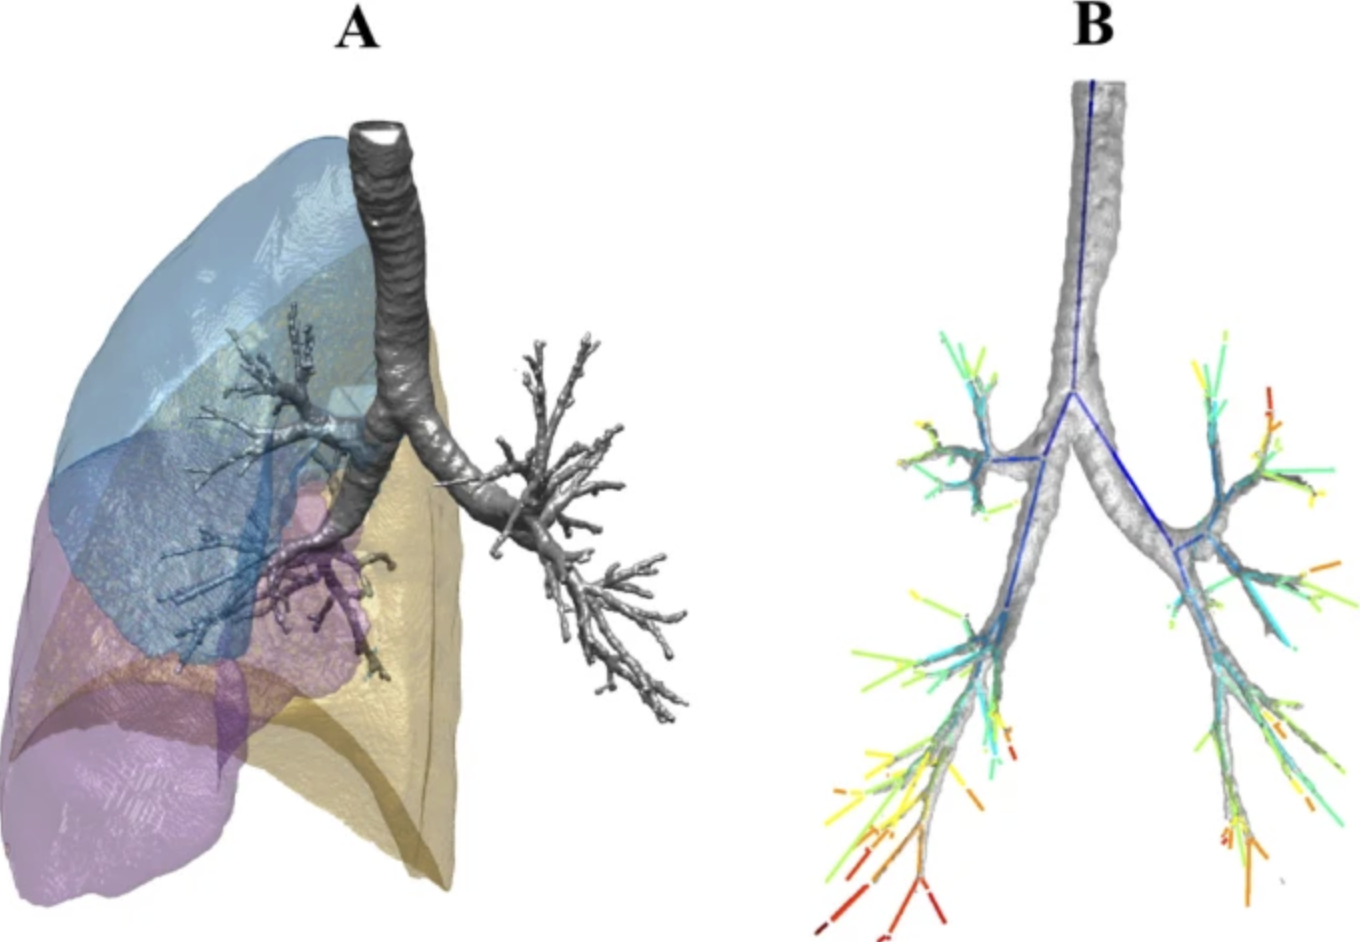
\includegraphics[scale=0.5]{lungs}
			 \caption{The kind of digital images we'd like to examine. \cite{belchi_lung_2018}}
		\end{figure}
		
	
		
		 With Persistent Homology, we have several invariants at our disposal that are resistant to common pitfalls with digital images like noise. The main invariants being the Persistent Homology Groups of course, but we also have Persistence Diagrams, and Euler Curves. So what exactly is Persistent Homology?
		 
		 In general, Persistent Homology is Algebraic Topology adapted to a sequence of spaces rather than a single space. This slight generalization is very powerful in that one can make precise the statement ``the important features are the ones that persist longer over different degrees of resolution". 
		 
		 Now, not unlike methods in machine learning and A.I., computing Persistent Homology is often expensive. There are standard procedures for accelerating the process of computing it, for example restricting to low dimensional persistence. In this project we explore other alternatives like projecting higher dimensional figures into lower dimensional planes, and computing the persistence of these projections. It seems reasonable to believe that there will be some connection between the persistence of these projections and that of the original higher dimensional figure. This is mainly due to the definition and properties of the PHT \cite{turner2014persistenthomologytransformmodeling} which uses a similar idea. PHT has a generalization XPHT \cite{turner_extended_2024} which we also wish to consider since it allows us to compute the persistence of a higher dimensional object through a codimension 1 object. Effectively reducing the dimension of our input by 1.
	
	
	\section*{Goals}
	
	I have a couple of goals for this first year:

		\begin{enumerate}
			\item Understand related literature.
			\item Master XPHT. Since it may be used to reduce computational complexity, mastering XPHT is useful towards the goal of more efficient computations.
			\item Create software that will handle XPHT for 3D images. 
			\item Understand the relationship between the persistence of higher dimensional objects with respect to lower dimensional objects related to them. 
			\item Explore the effects of segmentation on Persistent Homology. This goal is related to the accuracy part of my research question.
		\end{enumerate}
	
	I am currently well underway with many of these goals. I will explain the methodology below. 
	
	\section*{Methodology and Literature Review}
	
		For studying connectedness of digital images, one needs to make a choice of when to consider two regions being connected. It happens that the results vary depending on what one chooses, and the boundary of the image seems to be specially sensitive to this choice. To better understand the problem, I need to read \cite{Bleile_2022}.
		
		The main piece of software I am working on is a 3D version of a software created for 2D images in \cite{turner_extended_2024}. I need to completely understand the ideas there to be able to make an accurate program, as well as to prove that it works. The software depends on obtaining a surface mesh from a 3D object, for which an algorithm already exists. To understand the theoretical aspect, there is a comprehensive book \cite{wenger_isosurfaces_2013} that deals with it.
		
		My background on statistics is lacking for which I will be taking a Machine Learning course this summer in Sydney. AI and Persistent Homology are not mutually exclusive, one can use a combination of both methods to get better results. Having mastery over general AI concepts will be fruitful. I will attempt to audit afterwards a Computer Vision class, as well as a Differential Geometry class. Becoming stronger in statistics should help me explore the relationship between the persistence of higher dimensional objects with respect to ``partial lower dimensional" pictures of it. Similarly, Computer Vision should help me understand the effects of segmentation in general.
		
		There are several miscellanea papers that I am also reading ranging a wide variety of topics, from the effects of different resolutions on Persistent Homology, to generalizations of the PHT using tools from homotopy and sheaf theory. Having a wide area to draw ideas from is usually useful.
		
	
		
		\bibliography{refs}
	
	
	
\end{document}